\documentclass[12pt, titlepage]{article}
\usepackage{beamerarticle}
\usepackage[utf8]{inputenc}
\usepackage{hyperref}
\usepackage{amssymb,amsmath}

% Page settings
\usepackage[letterpaper, margin=1in]{geometry}
\usepackage{times}
%\usepackage{palatino}%\usepackage{lmodern, times}
%\usepackage{lmodern}%\usepackage{lmodern, times}
\usepackage{setspace}                           
\onehalfspacing %\doublespacing  % \singlespacing 

% Appendix
\usepackage{appendix}

% Line numbers
%\usepackage{lineno}
%\linenumbers


% Tables
\usepackage{array,booktabs,longtable,rotating}
\newenvironment{tablenotes}[1][]{
  \begin{minipage}{\textwidth}\emph{Notes:}{\footnotesize #1}
}{\end{minipage}}
\makeatletter
\def\fps@table{htbp}
\makeatother

% Graphics
\usepackage{graphicx,grffile}
\makeatletter
\def\maxwidth{\ifdim\Gin@nat@width>\linewidth\linewidth\else\Gin@nat@width\fi}
\def\maxheight{\ifdim\Gin@nat@height>\textheight\textheight\else\Gin@nat@height\fi}
\makeatother
% Scale images if necessary, so that they will not overflow the page
% margins by default, and it is still possible to overwrite the defaults
% using explicit options in \includegraphics[width, height, ...]{}
\setkeys{Gin}{width=\maxwidth,height=\maxheight,keepaspectratio}
% set default figure placement to htbp
\makeatletter
\def\fps@figure{htbp}
\makeatother

\usepackage{natbib}% plainnat
\bibliographystyle{abbrvnat}
\setcitestyle{authoryear,open={(},close={)}}
%\bibliographystyle{aer}


\setlength{\emergencystretch}{3em}  % prevent overfull lines
\providecommand{\tightlist}{%
  \setlength{\itemsep}{0pt}\setlength{\parskip}{0pt}}



\institute{}
\titlegraphic{}

\usepackage{xcolor}
\newcommand\todonote[1]{\textcolor{red}{#1}}



% Subscript
\newcommand\sub[1]{_{#1}}
\newcommand\supsc[1]{^{#1}}

\title{Notes on HeroX project}
\date{\today}

\begin{document}
\maketitle


% Todo notes
%\usepackage[textsize=tiny]{todonotes}
%\newcommand\redmarginpar[1]{\marginpar{\footnotesize{\textcolor{red}{#1}}}}
%\listoftodos[Notes]
\clearpage

\begin{figure}
\centering
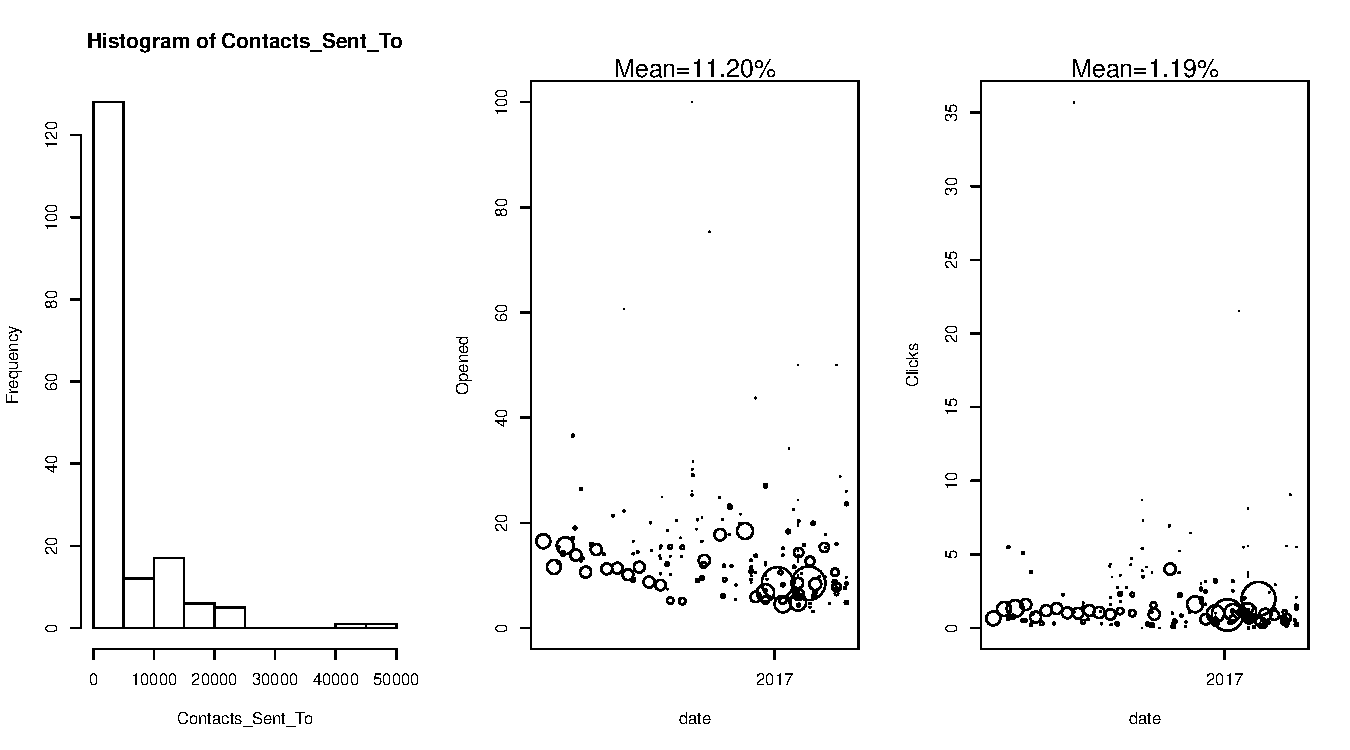
\includegraphics{report_notes_files/figure-latex/unnamed-chunk-2-1.pdf}
\caption{Contacts sent to, emails opened, clicks.}
\end{figure}

\newpage

\begin{figure}
\centering
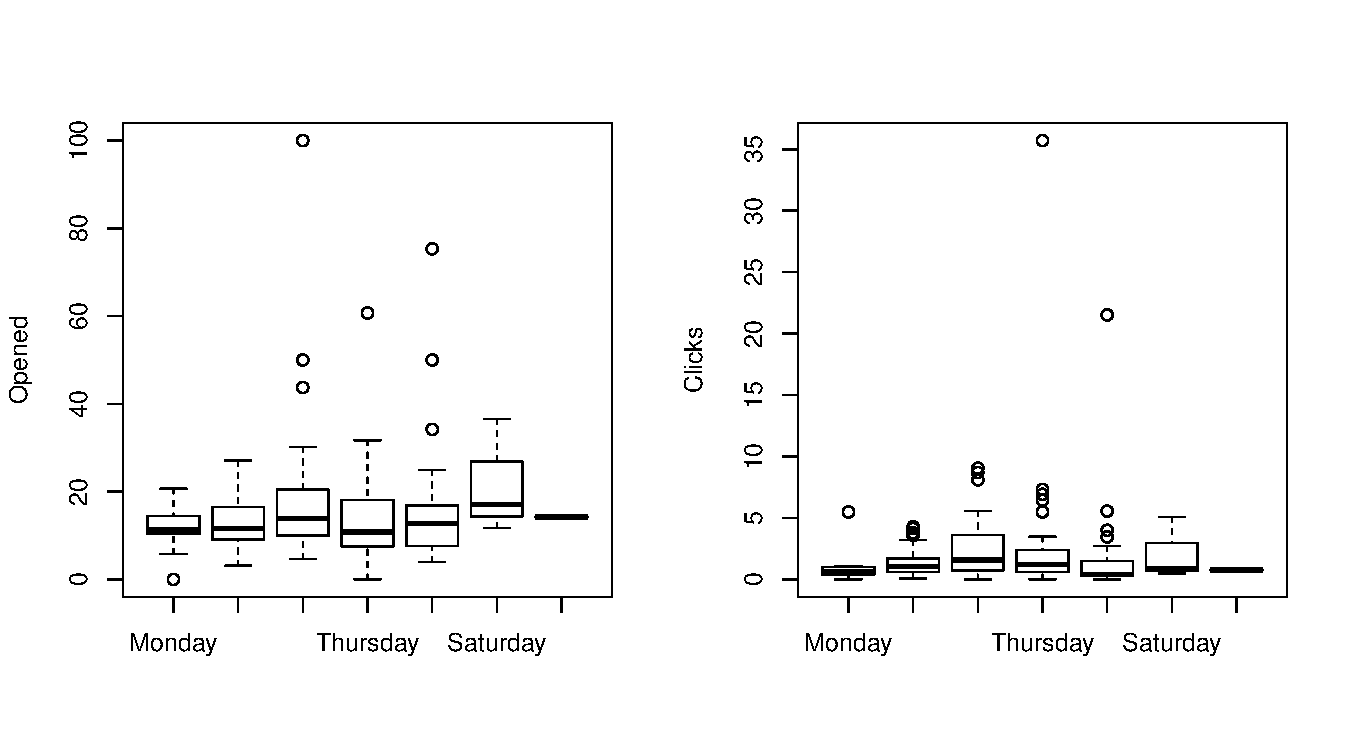
\includegraphics{report_notes_files/figure-latex/unnamed-chunk-3-1.pdf}
\caption{Days of the week}
\end{figure}

\newpage

\begin{verbatim}
## 
## Call:
## lm(formula = Opened ~ wdays + sender + contacts_qtl, weights = Contacts_Sent_To)
## 
## Weighted Residuals:
##     Min      1Q  Median      3Q     Max 
## -895.35 -185.59  -25.23  129.24 1108.46 
## 
## Coefficients:
##                                 Estimate Std. Error t value Pr(>|t|)    
## (Intercept)                      21.3115     5.0369   4.231 3.98e-05 ***
## wdaysTuesday                     -0.2467     2.9371  -0.084  0.93318    
## wdaysWednesday                   -0.1243     2.8906  -0.043  0.96576    
## wdaysThursday                    -1.9698     2.9151  -0.676  0.50022    
## wdaysFriday                      -0.3562     3.0250  -0.118  0.90641    
## wdaysSaturday                     7.6469     4.8809   1.567  0.11923    
## wdaysSunday                       3.1772     5.5388   0.574  0.56706    
## senderLiz                        -4.2471     3.0070  -1.412  0.15985    
## senderMaureen                    -0.8274     2.2901  -0.361  0.71839    
## senderNidhi                      -1.5327     2.9236  -0.524  0.60085    
## contacts_qtl(683,1.72e+03]       -5.3408     3.9946  -1.337  0.18319    
## contacts_qtl(1.72e+03,4.96e+03]  -6.2627     3.7495  -1.670  0.09690 .  
## contacts_qtl(4.96e+03,4.56e+04]  -9.4913     3.6359  -2.610  0.00994 ** 
## ---
## Signif. codes:  0 '***' 0.001 '**' 0.01 '*' 0.05 '.' 0.1 ' ' 1
## 
## Residual standard error: 351.4 on 154 degrees of freedom
## Multiple R-squared:  0.1454, Adjusted R-squared:  0.07877 
## F-statistic: 2.183 on 12 and 154 DF,  p-value: 0.01501
\end{verbatim}

\begin{verbatim}
## 
## Call:
## lm(formula = Clicks ~ wdays + sender + contacts_qtl, weights = Contacts_Sent_To)
## 
## Weighted Residuals:
##     Min      1Q  Median      3Q     Max 
## -133.01  -31.71   -5.89   19.16  348.32 
## 
## Coefficients:
##                                 Estimate Std. Error t value Pr(>|t|)    
## (Intercept)                      3.10165    0.89708   3.458 0.000705 ***
## wdaysTuesday                    -0.22239    0.52309  -0.425 0.671324    
## wdaysWednesday                   0.06039    0.51483   0.117 0.906766    
## wdaysThursday                   -0.03675    0.51918  -0.071 0.943662    
## wdaysFriday                     -0.04405    0.53875  -0.082 0.934946    
## wdaysSaturday                    0.56438    0.86929   0.649 0.517149    
## wdaysSunday                     -0.47362    0.98646  -0.480 0.631824    
## senderLiz                       -0.30901    0.53555  -0.577 0.564780    
## senderMaureen                    0.51875    0.40787   1.272 0.205341    
## senderNidhi                      0.93975    0.52070   1.805 0.073061 .  
## contacts_qtl(683,1.72e+03]      -1.89901    0.71143  -2.669 0.008417 ** 
## contacts_qtl(1.72e+03,4.96e+03] -2.45798    0.66779  -3.681 0.000321 ***
## contacts_qtl(4.96e+03,4.56e+04] -2.38678    0.64755  -3.686 0.000315 ***
## ---
## Signif. codes:  0 '***' 0.001 '**' 0.01 '*' 0.05 '.' 0.1 ' ' 1
## 
## Residual standard error: 62.58 on 154 degrees of freedom
## Multiple R-squared:  0.1612, Adjusted R-squared:  0.09588 
## F-statistic: 2.467 on 12 and 154 DF,  p-value: 0.005649
\end{verbatim}

\newpage

\begin{figure}
\centering
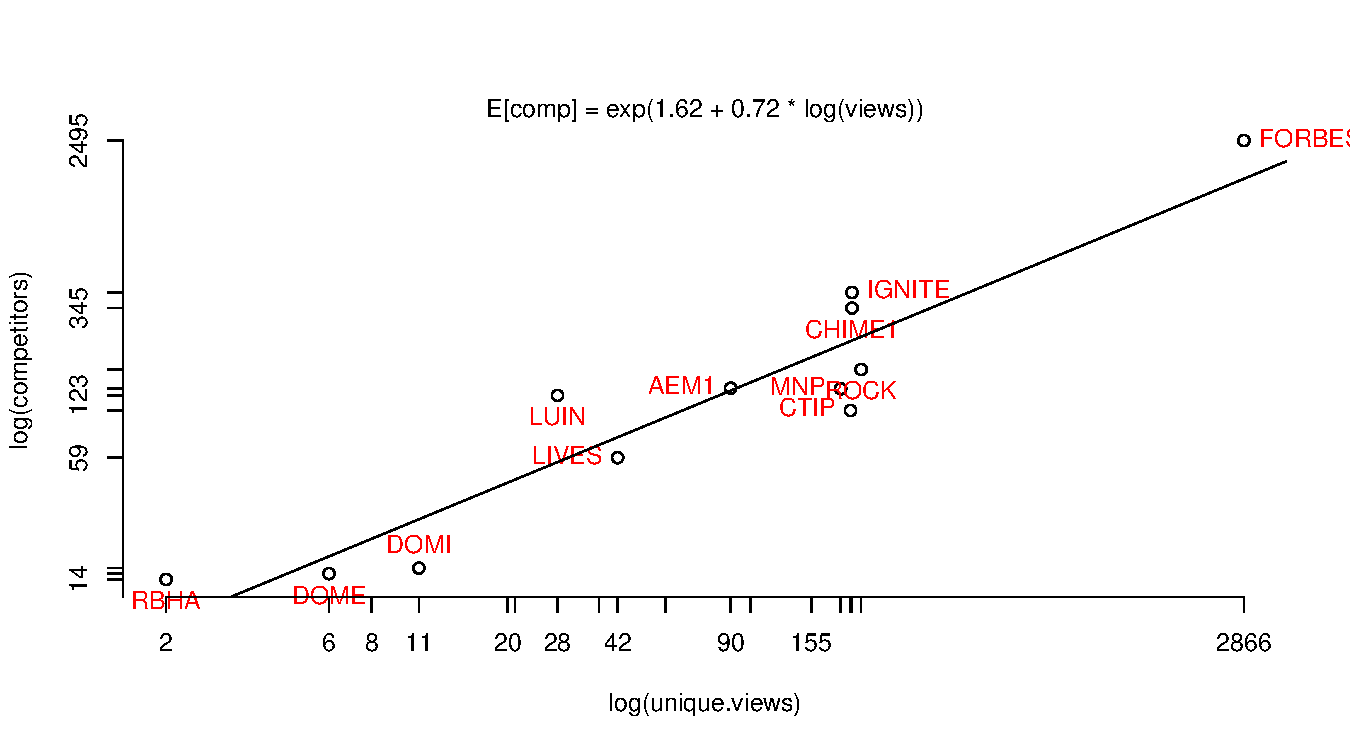
\includegraphics{report_notes_files/figure-latex/unnamed-chunk-5-1.pdf}
\caption{Relationship between competitors and unique visits.}
\end{figure}

\begin{figure}
\centering
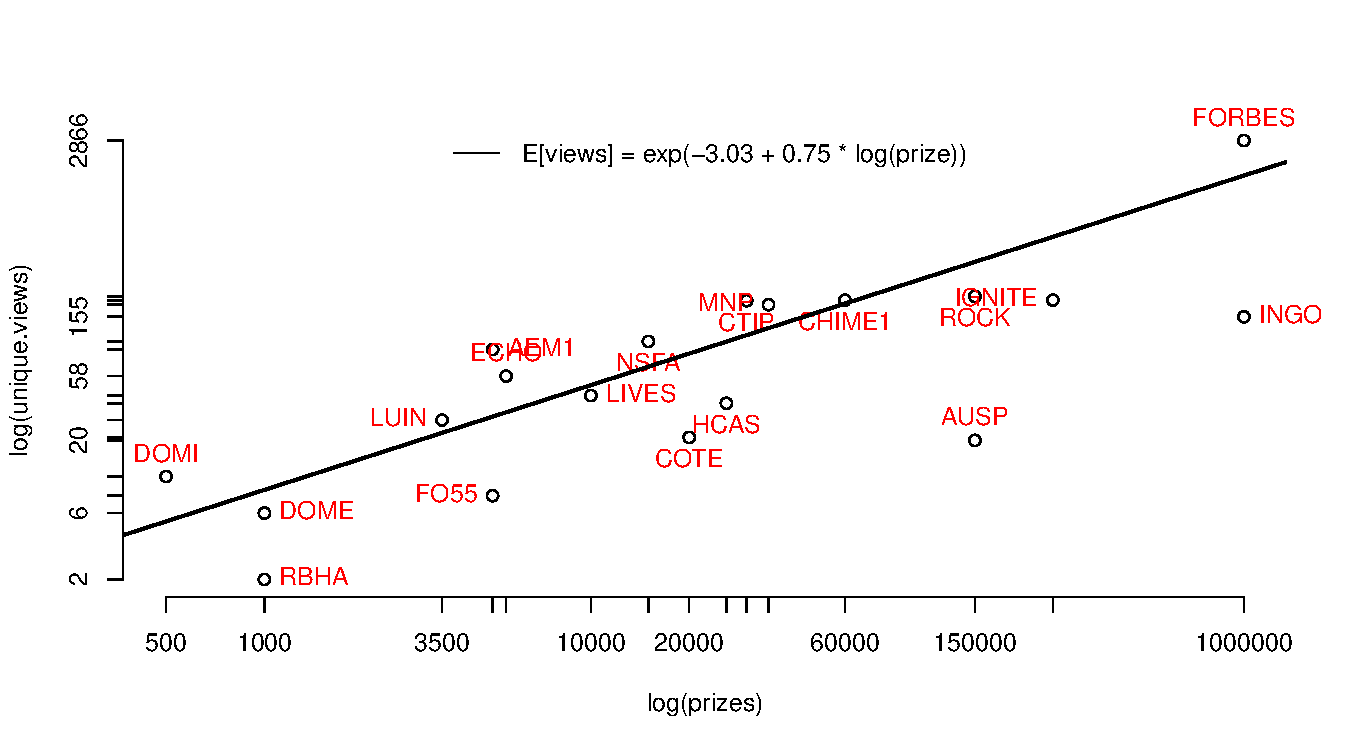
\includegraphics{report_notes_files/figure-latex/unnamed-chunk-6-1.pdf}
\caption{Relationship between prize pool and unique visits.}
\end{figure}

\bibliography{library.bib}

\end{document}